\section{PM10 Monitoring, Interpolation and Visualization System}
\label{sec: imple}

The methodologies and implementation details concerning the systems developed in this work are presented and explained in this section.

\subsection{PM10 Monitoring System Assembly}

The low-cost PM10 monitoring system consist of a PM10 sensor, a microcontroller board with a NB-IoT chipset and a step-up voltage converter.
The PM10 sensor used was the PMS5003, a low-cost light-scattering optical sensor, which outputs its measures through a digital signal, processed by a microprocessor in real-time. It operates in temperatures between -10ºC and 60ºC, and relative humidity from 0 to 99\%.

The development board used was SODAQ SFF R412M, which has low power consumption and allows the use of both NB-IoT and LTE-M technologies. It contains an integrated micro-controller, the Atmel SAMD21, which allows it to be programmed through the same
tools as Arduino compatible boards.

Subscriber identity module cards provided by the mobile operators NOS and Altice Portugal were used for this board NB-IoT remote communications. These card were previously configured by the mobile operators according to the specifications needed for its optimal use in NB-IoT devices. AT commands are used to communicate through the NB-IoT module. The commands used in the implementation of the developed system, and in the micro-controller program, along with its purpose are presented in Table \ref{table:atCommands}.

\begin{table}[ht]
\footnotesize
\centering
\caption{AT commands used with the NB-IoT micro-controller.}
\label{table:atCommands}
\begin{tabular}{l>{\raggedright\arraybackslash}p{0.33\textwidth}} % centered columns (4 columns)
\toprule
Command&Functionality\\
\midrule
AT+CFUN&Set the mobile terminal on\\
AT+CGATT&GPRS Attach\\
AT+USOCR&Create a socket\\
AT+USOST&Write to a remote address\\
AT+USOCL&Close socket\\
\bottomrule
\end{tabular}
\end{table}

The resulting system is presented in Figure \ref{fig:ieec5}. Two holes were made in the enclosure box to allow the airflow in the inlet and outlet of the sensor.

The development board was programmed, through the Arduino IDE, to collect data from the sensor, calculate 15 minute averages and send them to a server, which stores them in a database, replicating the behaviour of official monitoring networks systems. The server was developed in python, with the usage of UDP sockets, and the used database was MongoDB. 

\begin{figure}[ht]
\centering
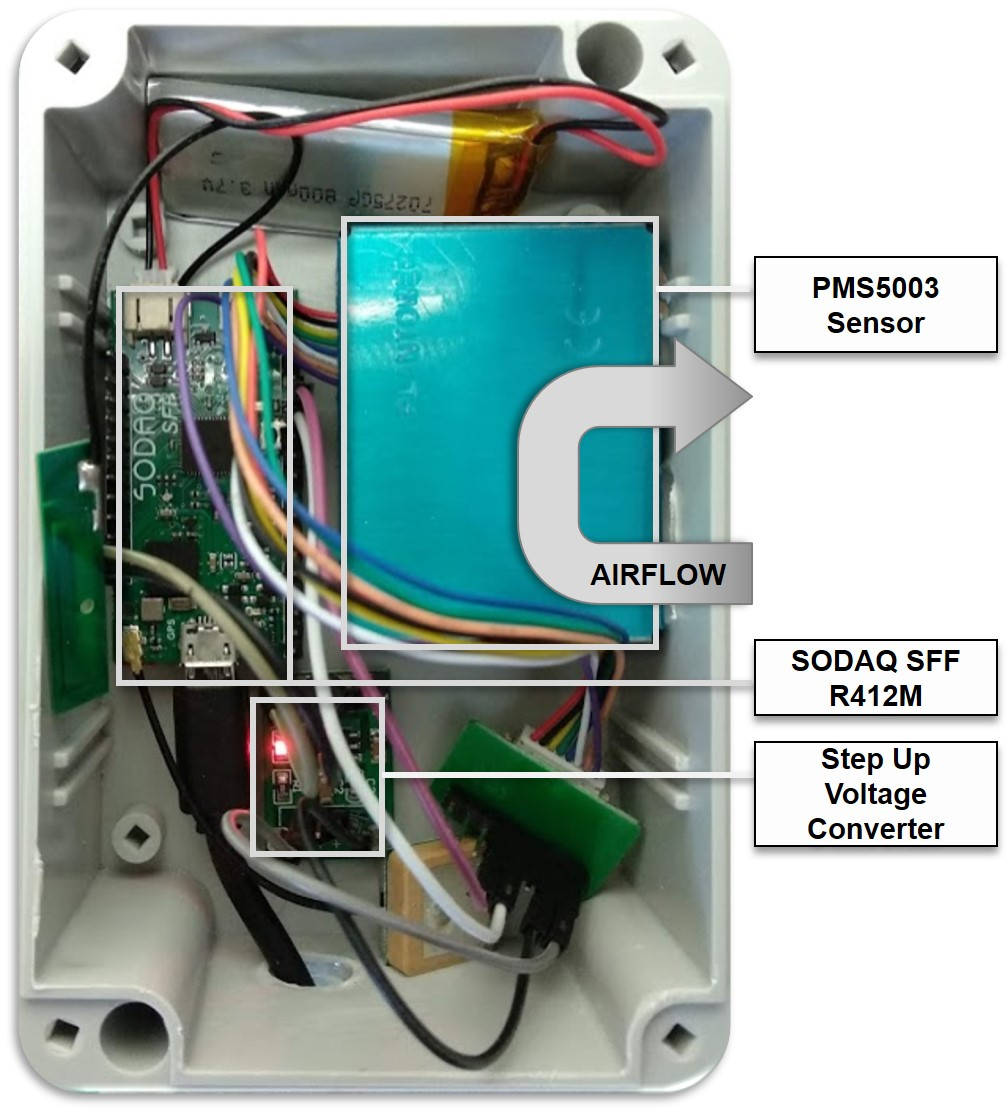
\includegraphics[width=0.49\textwidth]{./Images/circuit-final.jpg}
\caption{Developed PM monitoring system.}
\label{fig:ieec5}
\end{figure}

\subsection{Dataset Selection}

Only data from 2013 to 2017 was collected from Portuguese Online Database on Air Quality (QualAr) database, since it is the most consistent, with measures from the considered stations at high percentages of completeness.

Data was filtered to only concern monitoring stations in the greater area of Lisbon, since that is the area where these have the most spatial density in Portugal. The air quality monitoring network in the greater area of Lisbon is composed of 14 monitoring stations. Only 13 of these have operating PM10 sensors, and only 4 have operating PM2.5 sensors, with several of these lacking registered data in some years. The stations considered in this work are presented in Table \ref{table:completeness}.

\begin{table}[!htbp]
\footnotesize
\centering
\caption{Lisbon PM10 stations characterization and completeness in the dataset.}
\label{table:completeness}
\begin{tabular}{l>{\centering}p{0.06\textwidth}>{\centering}p{0.07\textwidth}>{\centering\arraybackslash}p{0.07\textwidth}}
\toprule
\multirow{2}{*}{Station}&\multirow{2}{*}{ID}&\multicolumn{2}{c}{Completeness (\%)}\\\cline{3-4}
&&Overall&Filtered\\
\midrule
Alfragide/Amadora&ALF&1.40&2.85\\
Alverca&ALV&97.47&99.96\\
Avenida da Liberdade&AVL&96.49&99.21\\
Entrecampos&ENC&76.40&99.50\\
Loures-Centro&LOC&85.88&91.46\\
Mem Martins&MEM&88.31&99.72\\
Odivelas-Ramada&ODI&82.89&98.88\\
Olivais&OLI&93.74&99.54\\
Quinta do Marquês&QMA&89.30&99.55\\
Reboleira&REB&68.88&96.88\\
Restelo&RES&29.66&40.81\\
Santa Cruz de Benfica&SCB&48.67&82.00\\
\bottomrule
\end{tabular}
\end{table}%

Further filtering was applied, data from the stations in Alverca and Alfragide was removed, due to lack of completeness in the dataset and sparse positioning, respectively. 

The objective of increasing percentages of data completeness, for every station in the dataset, was accomplished with the results of Table \ref{table:completeness}. The final dataset contained data regarding 11 657 time intervals.
%, as presented in Figure %\ref{fig:dataset-filtering}, corresponding to %the same number of total hours of PM10 %measurement of the Lisbon monitoring network.
%
%\begin{figure}[ht]
%\centering
%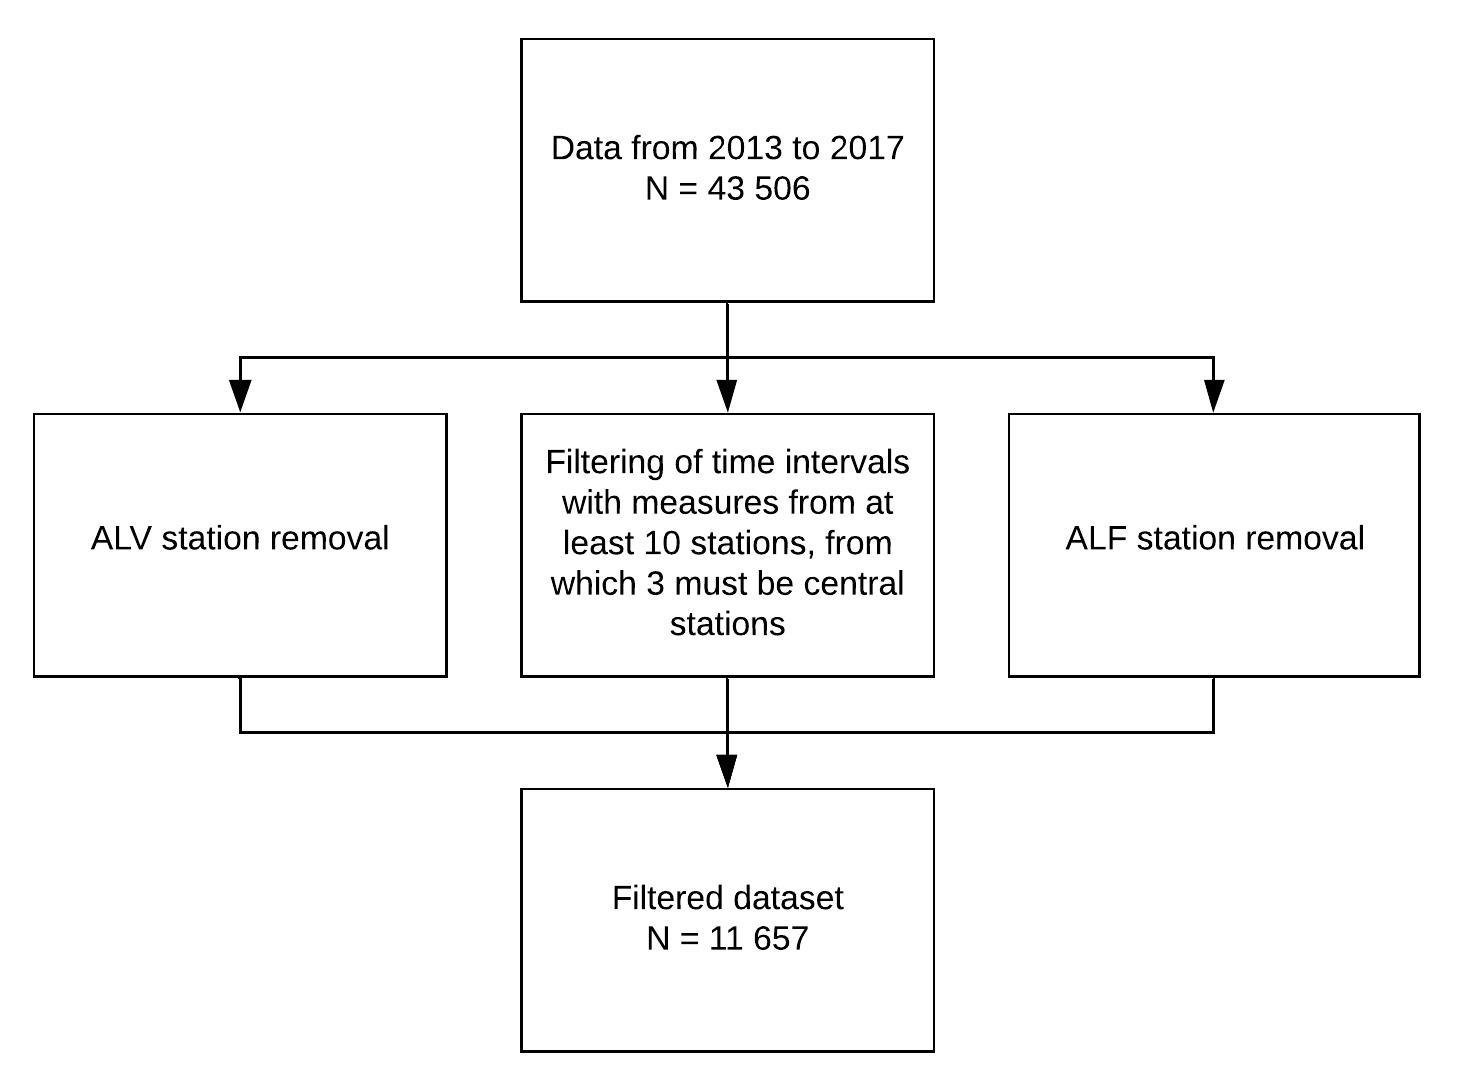
\includegraphics[width=0.49\textwidth]{./Images%/dataset-filtering.jpeg}
%\caption{Dataset exclusion process.}
%\label{fig:dataset-filtering}
%\end{figure}

The geographical location of the stations chosen for algorithm testing can be observed in Figure \ref{fig:map-filtered}, as well as, in red, the stations which are in the inside of the network outline, which will be used as infer targets.

\begin{figure}[ht]
\centering
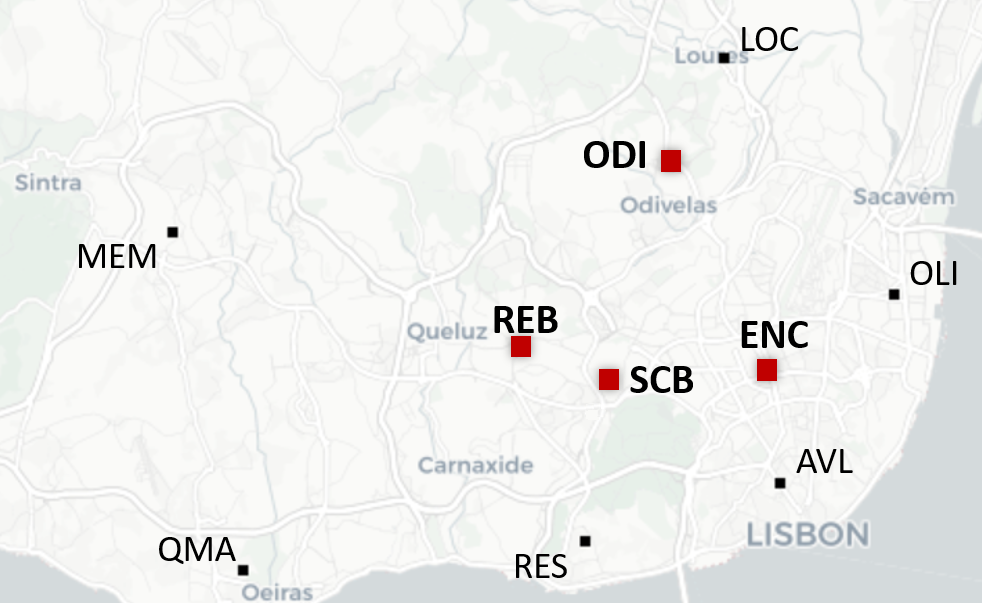
\includegraphics[width=0.46\textwidth]{./Images/map-filtered.png}
\caption{Selected stations, in the greater area of Lisbon.}
\label{fig:map-filtered}
\end{figure}

In the final filtered dataset, the Pearson coefficient was calculated between every station and every inference target station, as one can see in Table \ref{table:correlation-coef}. Possible resulting values vary from 1 to -1, where 1 represents total positive linear correlation, 0 represents no linear
correlation, and -1 total negative linear correlation.

\begin{table}[!htbp]
\centering
\footnotesize
\caption{Pearson correlation coefficients between stations.}
\label{table:correlation-coef}
\begin{tabular}[t]{l>{\centering}p{0.15\linewidth}>{\centering}p{0.15\linewidth}>{\centering}p{0.15\linewidth}>{\centering\arraybackslash}p{0.15\linewidth}}
\toprule
&ENC&ODI&REB&SCB\\
\midrule
%ALF&1&0.53&0.47&0.42&0.54\\
%ALV&0.76&0.78&0.79&0.69\\
AVL&0.83&0.77&0.78&0.76\\
ENC&1&0.84&0.82&\textbf{0.81}\\
LOC&0.77&0.79&0.79&0.69\\
MEM&0.77&0.78&0.8&0.66\\
ODI&\textbf{0.84}&1&\textbf{0.86}&0.78\\
OLI&0.83&0.76&0.78&0.74\\
QMA&0.77&0.78&0.83&0.71\\
REB&0.82&\textbf{0.86}&1&0.8\\
RES&0.76&0.83&0.81&0.73\\
SCB&0.81&0.78&0.8&1\\
\bottomrule
\end{tabular}
\end{table}%

\subsection{Algorithm Implementation}

Algorithms considered in this work for spatial interpolation were IDW, OK, Linear Interpolation (LI), Nearest Neighbors (NN) and FBNs.
In order to assess algorithm performance, cross validation tests were applied to the selected stations.
In each iteration, one measure from each central station (Figure \ref{fig:map-filtered}) was inferred using the readings
from remaining stations taken at the same time. In Algorithm \ref{main-pseudocode}, the pseudo-code of the setup of this process is presented.

\begin{algorithm}[!htbp]
\footnotesize
\linespread{1.15}\selectfont
\SetAlgoLined
 dataset = extractDataset()\;
 stations = stationsData()\;
 centralStations = centralStationsData()\;
 \ForEach{set in dataset}{
  \ForEach{station in stations}{
   \If{station in centralStations}{
    interpolationAlgorithms(station, set)\;
   }
  }
 }
 \caption{Algorithm execution setup.}
 \label{main-pseudocode}
\end{algorithm}

Both LI and NN were implemented with the python \textit{scipy} library \textit{interpolate} package. IDW was programmed in plain code without the use of any packages, due to its operations simplicity. 

Ordinary Kriging is the Kriging variant which was considered in this work, and it was implemented with the \textit{pykrige} python library. Kriging variograms can only be modelled if datasets have a relatively high number of points and high spatial density, which is not the case in these works experiments, in which observation points are few and sparsely distributed. 

Both IDW and OK were tested beforehand to find the most suitable user-defined parameters for their application in this work.

\subsubsection{Fuzzy Boolean Nets implementation}

FBNs have several implementation details which are user-defined and require analysis previous to its application.

\textbf{Antecedent and Consequent Areas}

PM10 concentration values and the coordinates (longitude and latitude) are the problem's variables. The coordinates, independent variables, were associated to two antecedent areas and the PM10 concentration, the dependent variable, was associated to one consequent area.

\textbf{Variables Scale Conversion}

Since each area only receives inputs between 0 and 1, a scale transformation was calculated for each area.

In the case of the coordinates, delimiting values were represented by the outline of the most exterior stations. The station at the extreme west location is Mem Martins and the extreme east station is Olivais. Therefore, the longitude defined value for 0 is -9.35 and for 1 is -9.1.

The same was done for the latitude. The southest station is Quinta do Marquês and the northest is Loures Centro. Consequently, the defined values for 0 and 1 for the antecedent area corresponding to the latitude coordinate are 38.69 and 38.83 respectively.

Finally, for the PM10 concentration values, the minimum value was 0 $\mu g/m^3$, and the maximum 175 $\mu g/m^3$, which is above the highest registered value in the filtered dataset.

\textbf{Parametrization}

Several other user-defined parameters were tested. These were the number of testing and training epochs, the network size, the granularity and the number of samples per neuron.

\subsubsection{Algorithm Performance Statistics}

In order to assess the results of the cross validation approach, the statistical error parameters presented in equations \eqref{mae} and \eqref{rmse} were used.

\begin{equation} 
\label{mae}
\scalebox{1.2}{ $ MAE = \dfrac{\sum_{i=1}^{n} |M_i - O_i|}{n}$}
\end{equation}

\begin{equation} 
\label{rmse}
\scalebox{1.2}{ $ RMSE = \sqrt[2]{\dfrac{1}{n}\sum_{i=1}^{n} {(M_i - O_i)}^{2}}$}
\end{equation}

%\begin{equation} 
%\label{r2}
%\scalebox{1.4}{ $ {R}^{2} = 1 - \dfrac{\sum_{i=1}^{n} {(O_i %- M_i)}^{2}}{\sum_{i=1}^{n} {(O_i - \overline{O_i})}^{2}}$}
%\end{equation}

Where $M_i$ represents the modelled value, $O_i$ represents the observed value and $n$ is the total of inferences.% and $\overline{O_i}$ is the mean of the observed values.

Maximum Absolute Error (MAE) measures the average magnitude of errors in a set of predictions. Root Mean Square Error (RMSE) is a quadratic parameter that also measures the average magnitude of the error.
Both express average model prediction error in units of the variable of interest, which for PM10 concentration are $\mu g/m^3$. Regarding RMSE, since errors are squared before they are averaged, increased weight is given to large errors.


\subsection{System for online data visualization}

The system for online data visualization is composed of a database and an html, css and javascript apache website with a javascript library which provides custom map web visualization and rendering, Mapbox GL JS.

\subsubsection{Database}

A MongoDB database was developed to store the values obtained by the monitoring systems. 

MongoDB was chosen for this specific application due to its high scalability and flexibity. Each database contains collections, which in turn contain documents. Documents are filled with fields and the size and content of documents in the same collection can vary.

The database used in this work only has one collection, in which every measure is saved, with corresponding date and time, and sensor ID. Despite the non-enforcement of document structures in the database, for the purpose of this work, each valid document must have fields for the date, location, sensor ID and PM10 value, and the set of date and sensor ID fields can not be repeated in different documents.

\subsubsection{Mapbox GL JS}

In this work, extrusion of polygons, provided by the Mapbox GL JS library, was used to represent the levels of estimated PM10 concentration values Extrusion height and color is determined by the pollution value at each location of the map.

For the representation of these extrusions, a convex hull was defined, delimited by the Lisbon monitoring station networks which are on the edges. This resulted in a grid with a resolution of 100 $m^2$. For these extrusions to be included, a geojson file was created, with the polygons of every element in the defined grid. A python script is running in the background which performs an hourly interpolation with the updated values, according to QualAr reports, and updates the geojson.

%Regarding the javascript implementation, a Map object, which represents the whole map visualization, is defined in the main website file. In the javascript code of the webpage, the geojson file, which should be saved in a local directory, is accessed, and its respective extrusions are inserted in the Map object which is rendered when users access the webpage.